\section{Using RKWard - an example RKWard session}
\label{sec:using_RKWard}
To see how RKWard works in practice an example session is described.
This might be a routinely used procedure on changing data stets or
\proglang{R} scripts which are complex and therfore
more conveniently used guided manner. We assume that an experimental
treatment was given to 20 test subjects and the values of the dependent
variable before and after the treatment should be compared. 

\subsection{Importing data}
\label{sec:importing_data}
The data was saved as or exported to CSV format for example from a
spread sheet application. RKWards import plugin can
comfortably read it into a new \proglang{R} object.
The import dialog (``File->Import->Import
format->Import Text / CSV data'') assists during the
selection of the data by a common point and click interface (Figure~\ref{fig:import_data}A). Within our
example ``comma'' and ``period'' were chosen via ``Quick mode'' as field
separator character and decimal point character respectively. RKWard
also takes care of name conflicts in the .GlobalEnv or suggests to
overwrite or use another name.

\code{read.csv(file=/media/software/experiment.txt, 
na.strings = NA, nrows = -1, skip = 0,
check.names = TRUE, strip.white = FALSE, blank.lines.skip = TRUE)}

Checking the ``Edit Object'' box will automatically open a data editor tab
showing the imported data (Figure~\ref{fig:import_data}B).

\begin{figure}[htp]
 \centering
 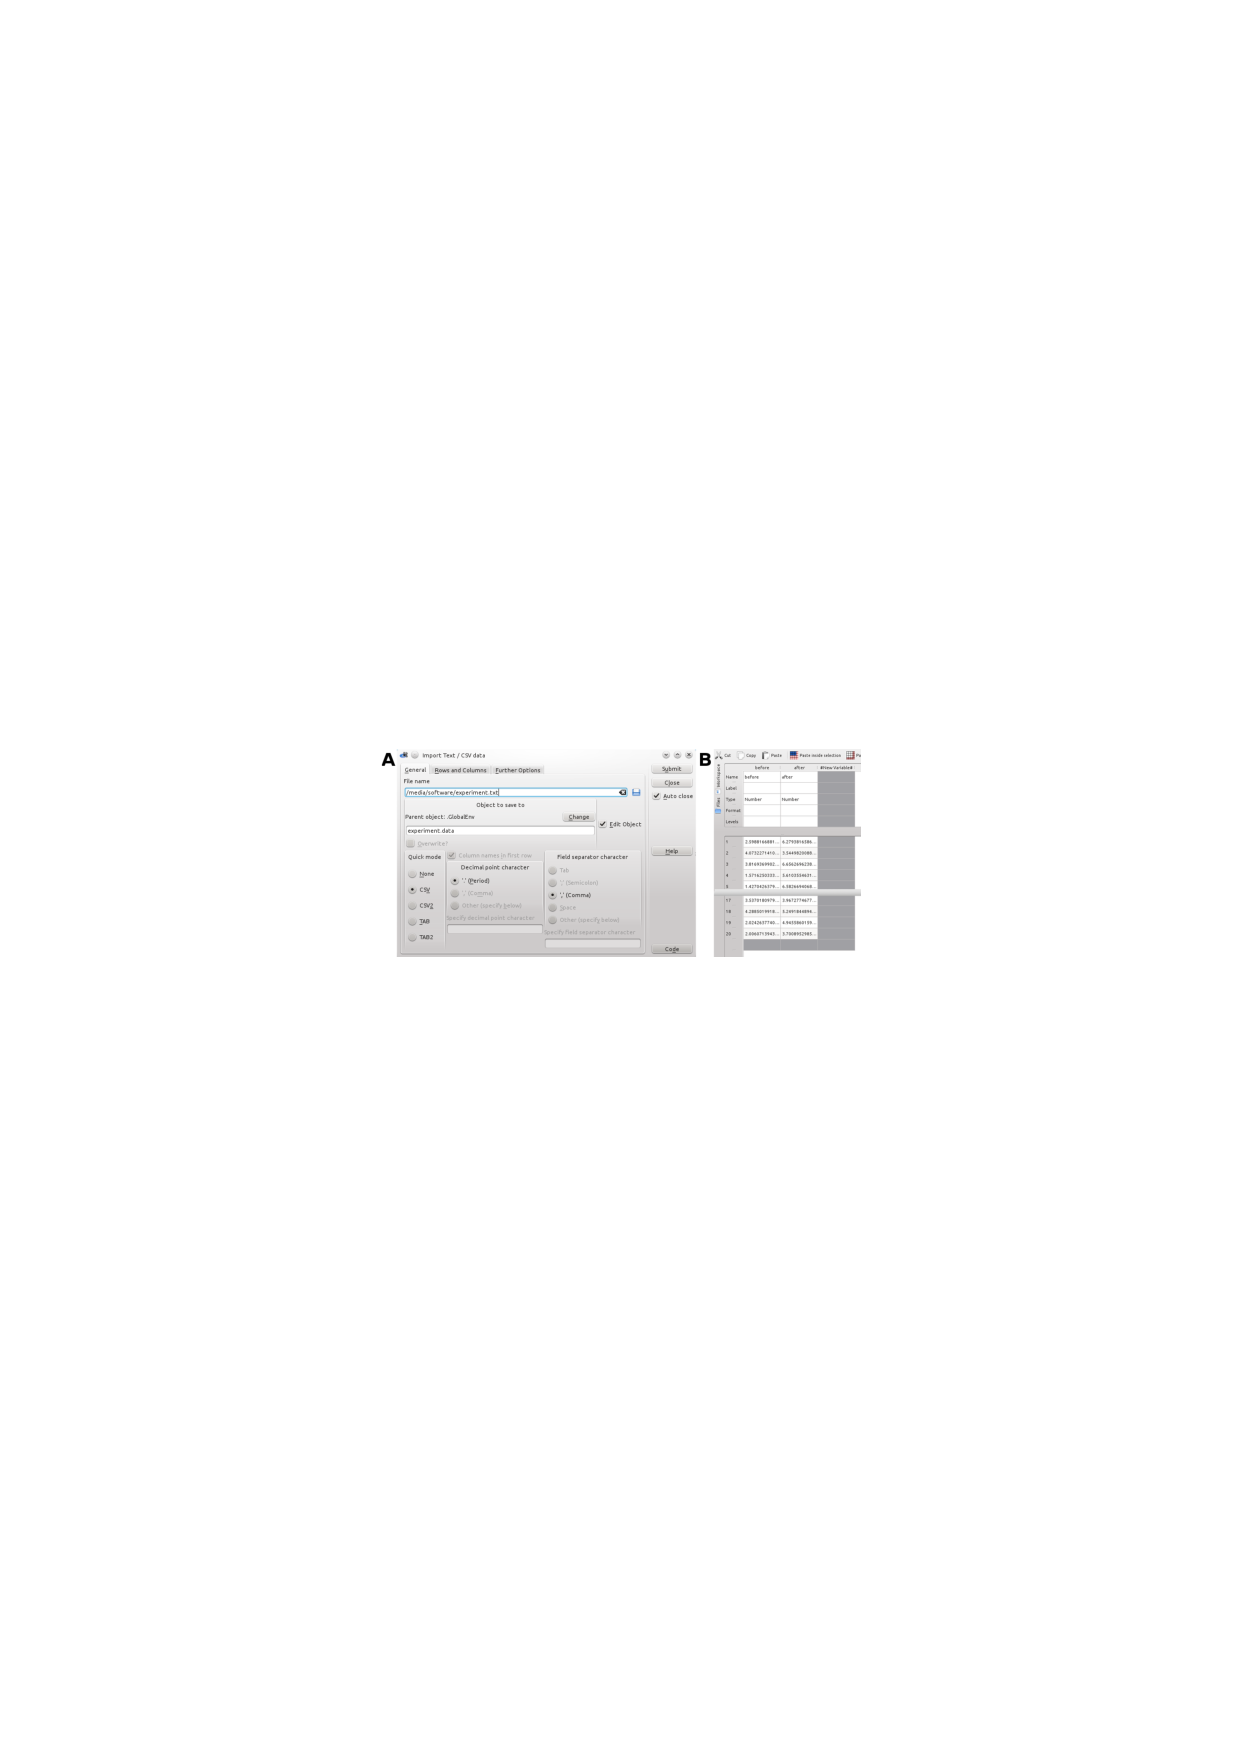
\includegraphics[clip=true,trim=0cm 5.7cm 0cm 5.7cm,width=16cm]{../figures/import_data.pdf}
 \caption{A) RKWard provides useful defaults
to import widely used data formats, including SPSS and Stata files. As
a common example the import of CSV data was chosen. B) Data editor. The imported CSV
data from experiment.txt are presented (data visually trimmed).}
 \label{fig:import_data}
\end{figure}

\subsection{Conducting a Student's t-test}
\label{sec:conducting_ttest}
To test the hypothesis that the given treatment significantly increased
the values of the dependent variable, a Students
t-test for a paired sample is applied. In the variable slot on the left
side you select the variables from the unfolded
\proglang{R} object (Figure~\ref{fig:t_test}A).

\begin{figure}[htp]
 \centering
 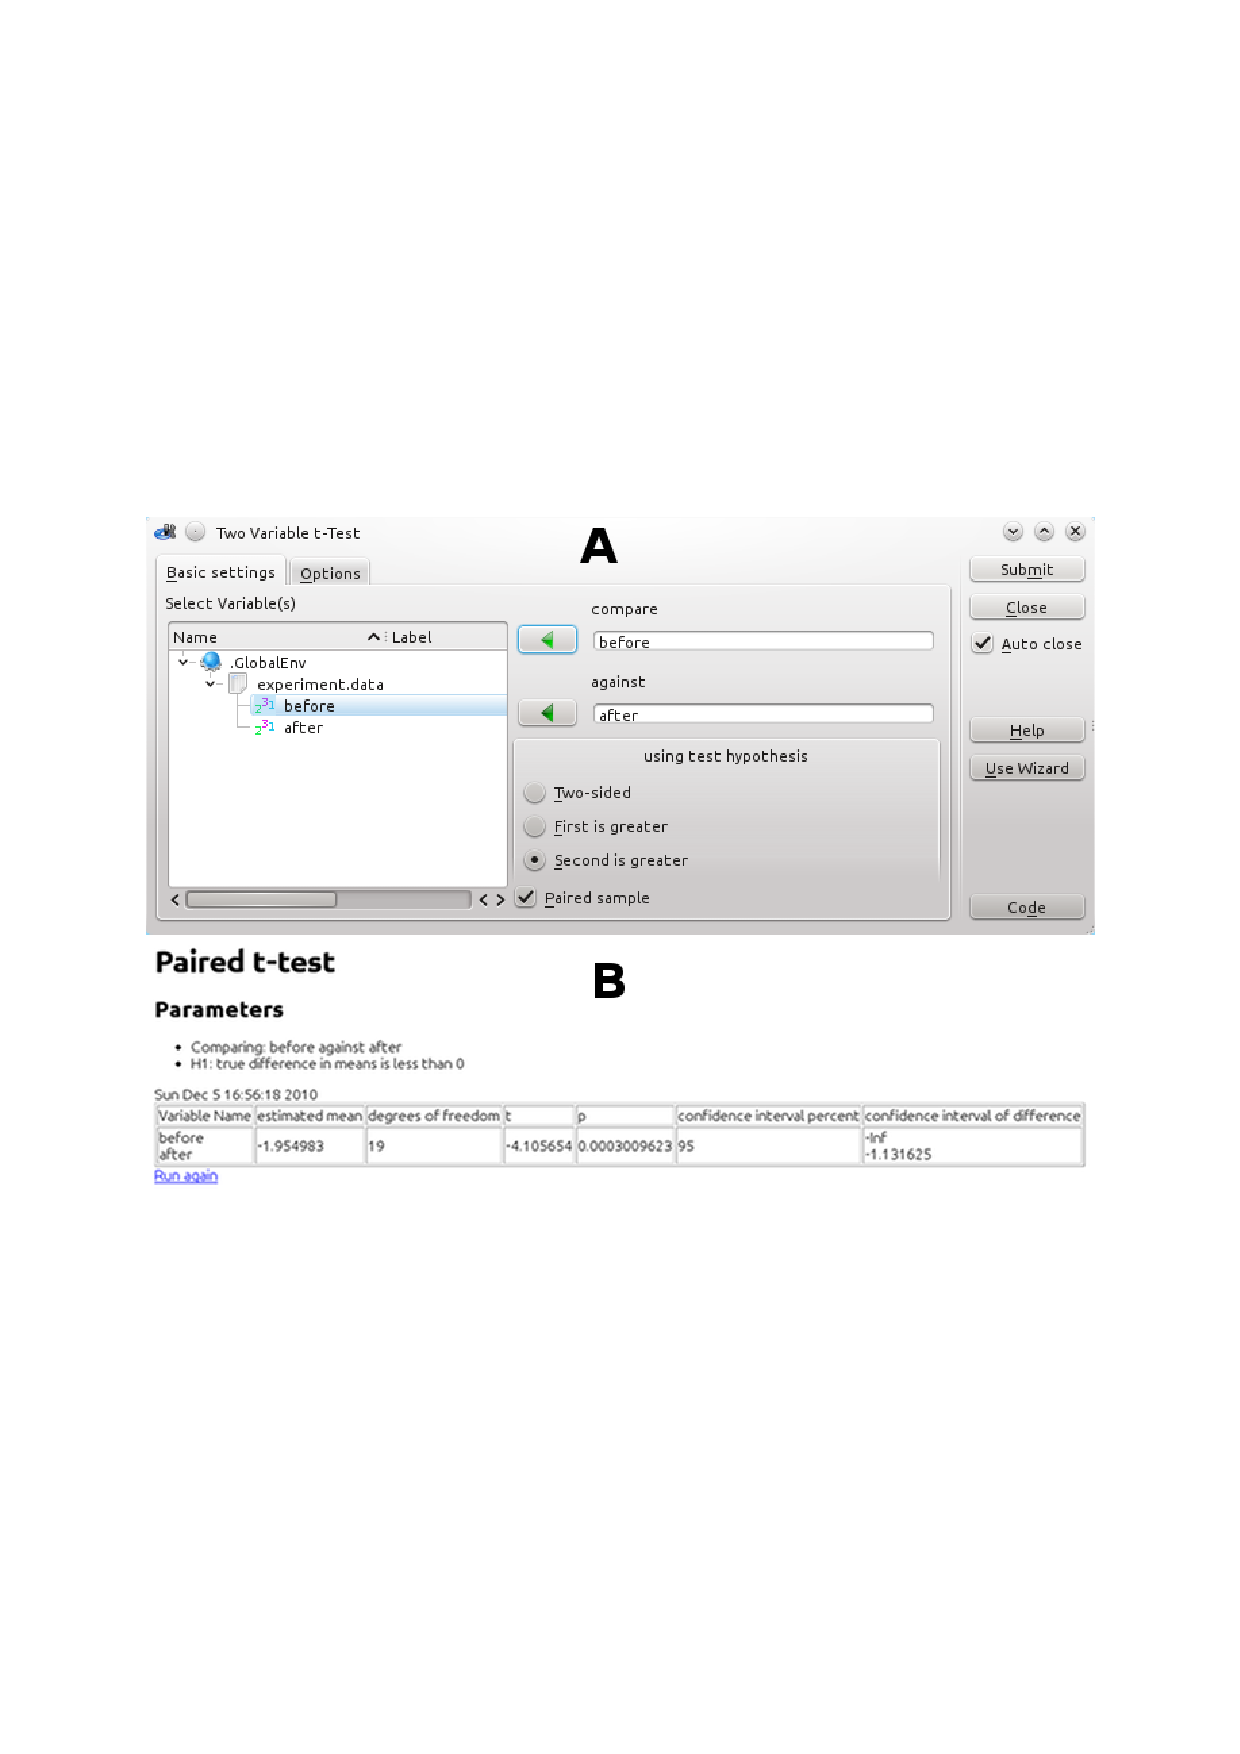
\includegraphics[clip=true,trim=0cm 5.7cm 0cm 5.7cm,width=16cm]{../figures/t-test.pdf}
 \caption{A) Students t-test dialog for a two variables. B) Test results in \proglang{HTML} format.}
 \label{fig:t_test}
\end{figure}

After the ``Submit'' button was pressed, RKWard opens the output document
to show the results (Figure~\ref{fig:t_test}B).

\subsection{Creating a plot}
\label{sec:create_plot}
To visualize the test data, ``Boxplot'' is chosen from the ``Plots'' menu
and variables selected like for the Students t-test.
The dialog allows to define custom variable labels (Figure~\ref{fig:boxplot1}).

Checking the ``Preview'' box will open a graphics window, show the plot as
it is configured and update the window on changes in real time. From
that window it can be exported directly to several data formats as
well (Figure~\ref{fig:boxplot2}).

\begin{figure}[htp]
 \centering
 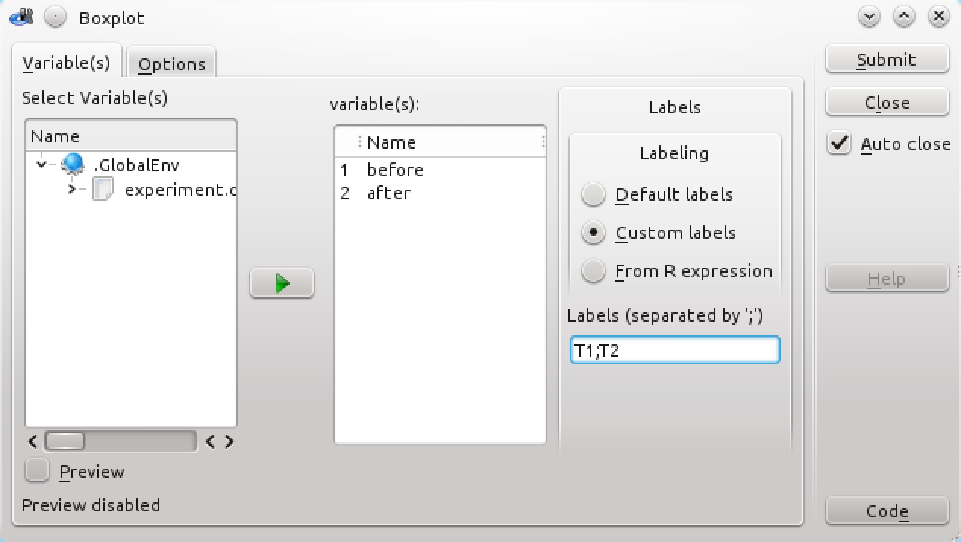
\includegraphics[clip=true,width=16cm]{../figures/boxplot1.pdf}
 \caption{Boxplot dialog.}
 \label{fig:boxplot1}
\end{figure}

\begin{figure}[htp]
 \centering
 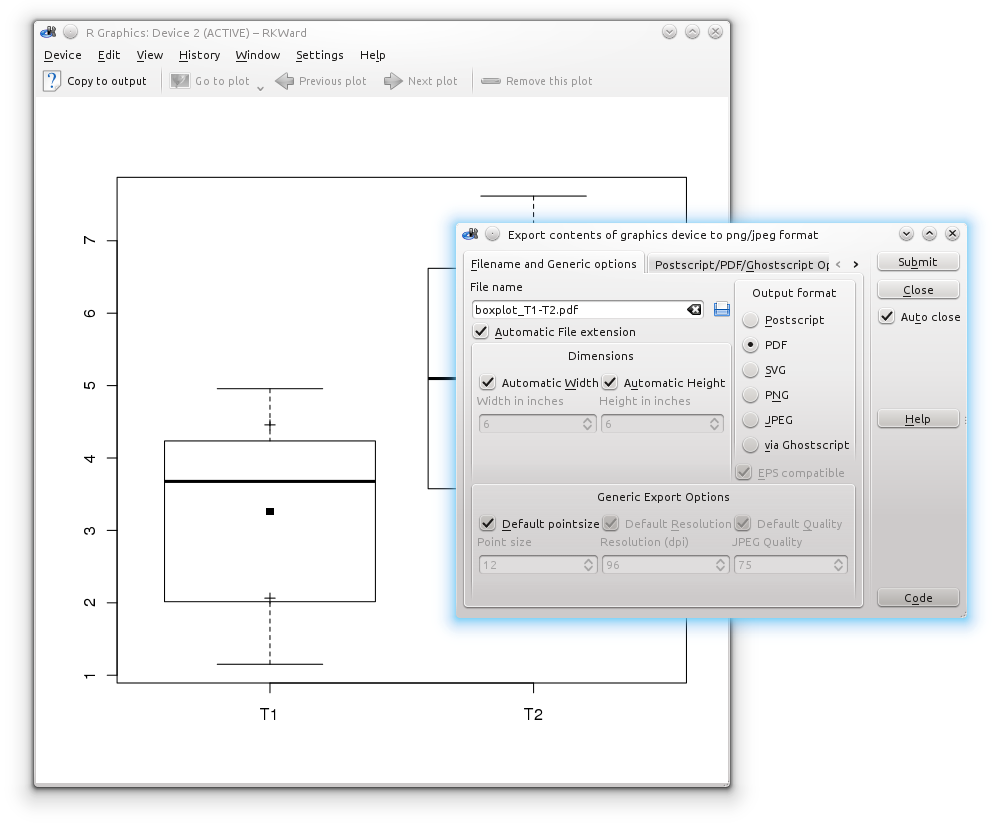
\includegraphics[clip=true,width=16cm]{../figures/boxplot2.pdf}
 \caption{Plotted data and plot export dialog.}
 \label{fig:boxplot2}
\end{figure}
